\documentclass[12pt, letterpaper]{article}
\usepackage[utf8]{inputenc}
\usepackage{geometry}
\geometry{
    a4paper,
    total={170mm,257mm},
    left=30mm,
    right=30mm,
    top=20mm,
}
\usepackage{subcaption} 
\usepackage{cite}
\usepackage{graphicx}
\usepackage{float}
\usepackage{amsmath}
\usepackage{amssymb}
\usepackage{algorithmic}
\usepackage{subcaption} 
\usepackage{fixltx2e}
\usepackage{stfloats}
\usepackage{hyperref}
\usepackage{url}
\usepackage{hyperref}
\usepackage{xcolor}
\usepackage{mathtools}
\newcommand{\minus}{\scalebox{0.75}[1.0]{$-$}}
\usepackage[utf8]{inputenc}
\usepackage[justification=centering,font=small]{caption}

\usepackage{appendix}

\usepackage{verbatim} % comments

\usepackage{booktabs}
\usepackage{siunitx}
\newcommand{\norm}[1]{\left\lVert#1\right\rVert}

\usepackage{color}
\usepackage{listings}
\lstset{language=Matlab,%
    basicstyle=\scriptsize\ttfamily,
    breaklines=true,
    tabsize=4,
    keepspaces=true,
    columns=flexible,
    %backgroundcolor=\color[gray]{0.9},
    framextopmargin=0pt,frame=single,
    %basicstyle=\color{red},
    morekeywords={matlab2tikz},
    keywordstyle=\color{blue},%
    morekeywords=[2]{1}, keywordstyle=[2]{\color{black}},
    identifierstyle=\color{black},%
    stringstyle=\color{mylilas},
    commentstyle=\color{mygreen},%
    showstringspaces=false,%without this there will be a symbol in the places where there is a space
    numbers=left,%
    numberstyle={\tiny \color{black}},% size of the numbers
    numbersep=9pt, % this defines how far the numbers are from the text
}
\usepackage{color} %red, green, blue, yellow, cyan, magenta, black, white
\definecolor{mygreen}{RGB}{28,172,0} % color values Red, Green, Blue
\definecolor{mylilas}{RGB}{170,55,241}

% correct bad hyphenation here
\hyphenation{op-tical net-works semi-conduc-tor}

\begin{document}

\title{Spacecraft Landing Trajectory Optimization}
\maketitle

\begin{table}[h]
\centering
\resizebox{\textwidth}{!}{%
\begin{tabular}{ccc}
Michael Spieler                 & Nicolas Gandar         & Nicolas Lesimple                     \\
Robotics and Autonomous Systems & Microengineering       & Computational Science \& Engineering \\
michael.spieler@epfl.ch         & nicolas.gandar@epfl.ch & nicolas.lesimple@epfl.ch            
\end{tabular}%
}
\end{table}

\begin{abstract}

In this paper we discuss trajectory optimization for propulsive spacecraft landing with minimal fuel consumption by formulating and solving a convex optimization problem using CVX and CVXPY software packages.
In a second part the minimal time trajectory and effects on fuel consumption are explored.

\end{abstract}

\section{Introduction}
%In 1997 NASA sent a rover to Mars which was expected to land within an ellipse $\SI{150}{\kilo\meter}$ across its major axis. The major reason for uncertainty was the use of parachutes to land. 

Convex optimization applied in control systems is an enabling technology for precision spacecraft landing.
In 2012 the Mars Science Laboratory (MSL) achieved the most accurate Martian landing within an ellipse of $20$ by $\SI{7}{\kilo\meter}$ using a powered descent stage \cite{bib:MSL}.
This technology allows companies like SpaceX to successfully recover and reuse the first stage of their Falcon9 rocket by a controlled propulsive landing with high precision.
In the following we discuss a minimal-fuel trajectory optimization problem for a simplified spacecraft model.

\section{Optimal spacecraft landing problem}

We consider exercise \textit{13.2 Optimal spacecraft landing} from the \textit{Additional Exercises for Convex Optimization} by Stephen Boyd and Lieven Vandenberghe \cite{Boyd:CVXcourse_extra_exercises} described in the following:

\subsection{Problem Description}
\label{sec:problem}

%We consider the problem of optimizing the thrust profile for a spacecraft to carry out a landing at a target position. This problem was taken from additional exercises part of the Convex Optimization course by Stephen Boyd \cite{Boyd:CVXcourse_extra_exercises}. 
We consider the problem of optimizing the thrust profile for a spacecraft to carry out a landing at a target position.
The spacecraft dynamics are
$$m\ddot{p} = f\minus mge_{3},$$ where $m > 0$ is the spacecraft mass, $p(t) \in \mathbb{R}^{3}$
is the spacecraft position, with 0 the target landing
position and $p_{3}(t)$ representing height, $f(t)\in \mathbb{R}^{3}$
is the thrust force, and $g > 0$ is the gravitational
acceleration. For simplicity we assume that the spacecraft mass is constant. This is not always
a good assumption, since the mass decreases with fuel use. We will also ignore any atmospheric
friction. We must have $p(T
^{td}) = 0$ and $p'(T^{td}) = 0$, where $T^{td}$ is the touchdown time. The
spacecraft must remain in a region given by
$$p_{3}(t) \geq \alpha \left\|(p_{1}(t), p_{2}(t))\right\|_{2},
$$ where $\alpha > 0$ is a given minimum glide slope. The initial position p(0) and velocity p'(0) are given. 

The thrust force $f(t)$ is obtained from a single rocket engine on the spacecraft, with a given
maximum thrust; an attitude control system rotates the spacecraft to achieve any desired direction
of thrust. The thrust force is therefore characterized by the constraint $\left\|f(t)\right\|_{2} \leq F^{max}$. The fuel use rate is proportional to the thrust force magnitude, so the total fuel use is
$$
\int_{0}^{T^{td}} \gamma \left\|f(t)\right\|_{2} dt,
$$
where $\gamma > 0$ is the fuel consumption coefficient. The thrust force is discretized in time, i.e., it is
constant over consecutive time periods of length $h > 0$, with $f(t) = f_{k}$ for $t \in [(k\minus 1)h, kh)$, for
k=1,...,K, where $T^{td} = Kh$. Therefore we have
$$v_{k+1} = v_{k} + (h/m)f_{k} \minus hge_{3},$$ $$p_{k+1} = p_{k} + (h/2)(v_{k} + v_{k+1}),$$
where $p_{k}$ denotes $p((k\minus 1)h)$, and $v_{k}$ denotes $p'((k\minus 1)h)$. We will work with this discrete-time model.
For simplicity, we will impose the glide slope constraint only at the times t = 0, h, 2h, . . . , Kh.

\subsection{Problem formulation}

The problem description above can be formulated mathematically in Problem \ref{eq:opt_problem}.
The decision variables are the position $\mathbf{p}$, velocity $\mathbf{v}$ and thrust $\mathbf{f}$ vectors at each of the $K$ time steps (Notation: bold letters for vectors, subscript for time index).
The function to minimize is the total fuel consumption as defined in section \ref{sec:problem}.
The constraints are: \textit{Max Thrust}, \textit{Glide Cone}, initial state, final state and discretized dynamics (same order as in Problem \ref{eq:opt_problem}).
We observe that all equality constraints are linear, and the inequality constraints can be formulated as second-order cone constraints.

\begin{equation}
\label{eq:opt_problem}
\begin{array}{lll}
  \underset{\mathbf{p,v,f}}{\mbox{minimize}} & \sum^{K}_{i=1} h \gamma \norm{\mathbf{f}_i}_2 & \\
  \mbox{subject to}
    & \norm{\mathbf{f}_i}_2 \leq F_{max} & i = 1,...,K \\
    & \mathbf{p}^z_i \geq \alpha \norm{\mathbf{p}^{x,y}_i}_2 & i = 1,...,K \\
    & \mathbf{p}_1 = \mathbf{p}_{init} & \\
    & \mathbf{v}_1 = \mathbf{v}_{init} & \\
    & \mathbf{p}_K = 0 & \\
    & \mathbf{v}_K = 0 & \\
    & \mathbf{v}_{i+1} = \mathbf{v}_i + \frac{h}{m} \mathbf{f}_i - hg\mathbf{e_3} & i = 1,...,K-1 \\
    & \mathbf{p}_{i+1} = \mathbf{p}_i + \frac{h}{2} (\mathbf{v}_i + \mathbf{v}_{i+1}) & i = 1,...,K-1 \\
\end{array}
\end{equation}

%Note that the constraints are only guaranteed to hold at the discretization time steps.

Table \ref{tab:param} lists the parameter values used for initial numerical evaluation.

\begin{table}[h!]   
    \centering
    \begin{tabular}{lll}
        \toprule
        Parameter & Value & Description \\
        \midrule
        $\gamma$ & 1.0 & Fuel consumption coefficient \\
        $\alpha$ & 0.5 & Glide cone slope \\
        $h$ & \SI{1.0}{\second} & Discretization time \\
        $K$ & 35 & Number of time steps \\
        $m$ & \SI{10}{\kilo\gram} & Mass \\
        $\mathbf{g}$ & \SI{0.1}{\meter/\second^2} & Gravity \\
        $F_{max}$ & \SI{10}{\newton} & Maximal thrust \\
        $\mathbf{p}_{init}$ & $\begin{bmatrix}50&50&100\end{bmatrix} \SI{}{\meter} $ & Initial position \\
        $\mathbf{v}_{init}$ & $\begin{bmatrix}-10&0&-10\end{bmatrix} \SI{}{\meter/\second} $ & Initial velocity \\
        \bottomrule
    \end{tabular}
    \caption{Parameter values and description}
    \label{tab:param}
\end{table}

\subsubsection{Convexity and SOCP formulation}
It is easy to show that problem \ref{eq:opt_problem} is convex.
The cost function is a sum of norms, which is convex.
The maximal thrust and glide cone constraints are quadratic and second-order cone constraints respectively, where both are convex.
Finally, the equality constraints are linear and are therefore convex as well. \cite{Boyd:CVXcourse}

By introducing a variable $\mathbf{t}$ we can reformulate the problem as a Second-Order Cone Program (SOCP) shown in \ref{eq:socp}.
There exist solvers that can solve SOCPs efficiently.
Our CVXPY implementation is using ECOS, an interior-point solver for second-order cone programming \cite{bib:Domahidi2013ecos}.
Finally, we notice that without the glide cone constraint, the problem could be formulated as a QCQP.

\begin{equation}
\label{eq:socp}
\begin{array}{lll}
  % \mbox{minimize} & \mathbf{1}^T t & \\
  \underset{\mathbf{p,v,f,t}}{\mbox{minimize}} & \mathbf{1}^T \mathbf{t} & \\
  \mbox{subject to}
    & \norm{\mathbf{f}_i}_2 \leq \mathbf{t}_i & i = 1...K \\
    & \norm{\mathbf{f}_i}_2 \leq F_{max} & i = 1...K \\
    & \norm{\mathbf{p}^{x,y}_i}_2 \leq \frac{1}{\alpha} \mathbf{p}^z_i & i = 1...K \\
    & \mathbf{p}_1 - \mathbf{p}_{init} = 0 & \\
    & \mathbf{v}_1 - \mathbf{v}_{init} = 0 & \\
    & \mathbf{p}_K = 0 & \\
    & \mathbf{v}_K = 0 & \\
    & \mathbf{v}_i - \mathbf{v}_{i+1} + \frac{h}{m} \mathbf{f}_i - hg\mathbf{e_3} = 0 & i = 1,...,K-1 \\
    & \mathbf{p}_i - \mathbf{p}_{i+1} + \frac{h}{2} (\mathbf{v}_i + \mathbf{v}_{i+1}) = 0 & i = 1,...,K-1 \\
\end{array}
\end{equation}

\section{Solution}

Using CVX we solve Problem \ref{eq:socp} using parameters from Table \ref{tab:param}. The resulting trajectory and thrust profile are studied in the following.
The Matlab code to solve the problem in CVX  can be found in the Appendix \ref{matlab_code}.

\subsection{Trajectory and Constraint analysis}

\begin{figure}[H]
  \begin{subfigure}[b]{0.5\textwidth}
    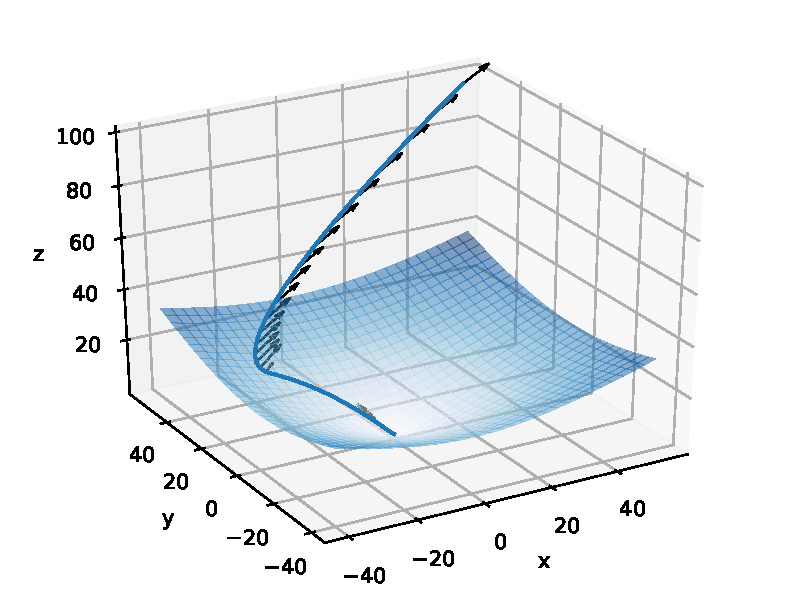
\includegraphics[width=\textwidth]{traj.pdf}
    \vspace{0.5cm}
    \caption{Spacecraft trajectory and thrust vectors with the glide cone constraint.}
    \label{fig:trajectory}
  \end{subfigure}
  %
  \begin{subfigure}[b]{0.5\textwidth}
    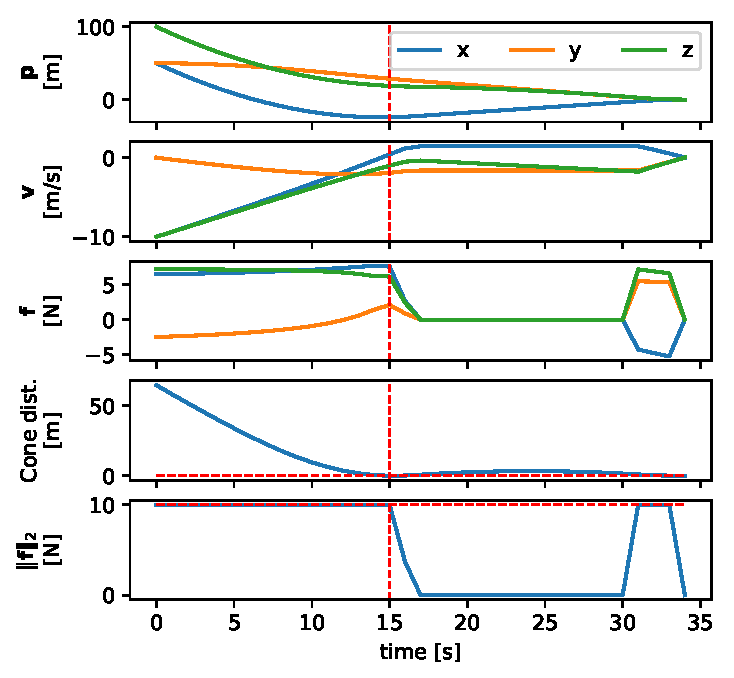
\includegraphics[width=\textwidth]{variables.pdf}
    \caption{Evolution of position, velocity and thrust with constraint margins}
    \label{fig:variables}
  \end{subfigure}
  \caption{Trajectory and variable evolution for $K=\SI{35}{\second}$.}
  \label{fig:trandandvariables}
\end{figure}


In Figure \ref{fig:trajectory}, we observe that the spacecraft starts by decelerating strongly to avoid leaving the allowed region. After almost touching the \textit{Glide Cone} constraint border, it enters a parabolic trajectory towards the target where no thrust is applied until a final burn shortly before touchdown.

\subsubsection{Constraint Activity}
In Figure \ref{fig:variables} we analyze the trajectory and thrust profile and the margins to the \textit{Max Thrust} and \textit{Glide Cone} constraints. One can visually verify that both constraints (in red) are always respected.

Figure \ref{fig:duals} shows the dual variables of \textit{Max Thrust} and \textit{Glide Cone} constraints. The corresponding constraint is active where the duals are non-zero, which supports the findings from Figure \ref{fig:trajectory}. The \textit{Max Thrust} constraint is active during deceleration until the spacecraft reaches the cone border, where thrust is turned off. It is active again for final deceleration. The \textit{Glide Cone} constraint is only active when approaching the cone at time $K=15$ and upon landing.

\begin{figure}[H]
    \centering
    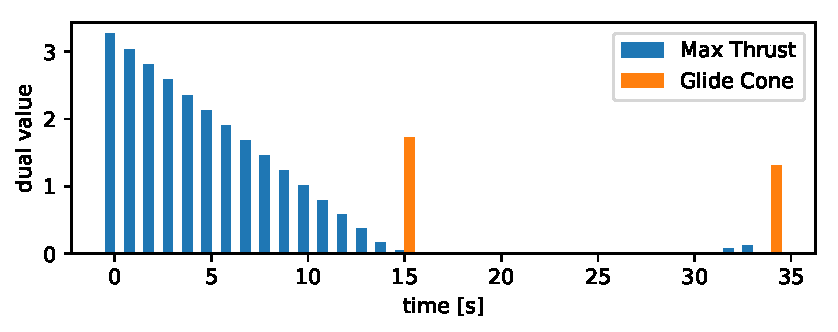
\includegraphics[width=0.7\textwidth]{duals.pdf}
    \caption{Dual variables of \textit{Max Thrust} and \textit{Glide Cone} constraints}
    \label{fig:duals}
\end{figure}

\subsection{Minimum Landing Time}
To find the minimum landing time we search for a minimal K for which Problem \ref{eq:socp} is still feasible.
This is achieved by iteratively decreasing K and solving the problem until it becomes infeasible.
Note: This can be done efficiently using binary search. The solution for $K_{min}=26s$ is shown in Figure \ref{fig:var26}.

\begin{figure}[H]
  \begin{subfigure}[b]{0.5\textwidth}
    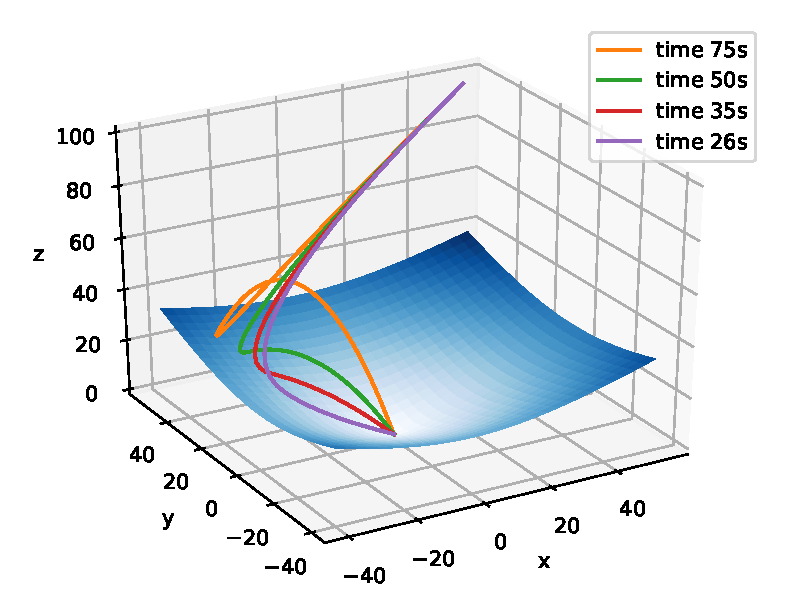
\includegraphics[width=\textwidth]{traj_multi.pdf}
    \vspace{0.5cm}
    \caption{Trajectories for different landing times. The shortest feasible time $K_{min}=\SI{26}{\second}$}
    \label{fig:traj_multi}
  \end{subfigure}
  %
  \begin{subfigure}[b]{0.5\textwidth}
    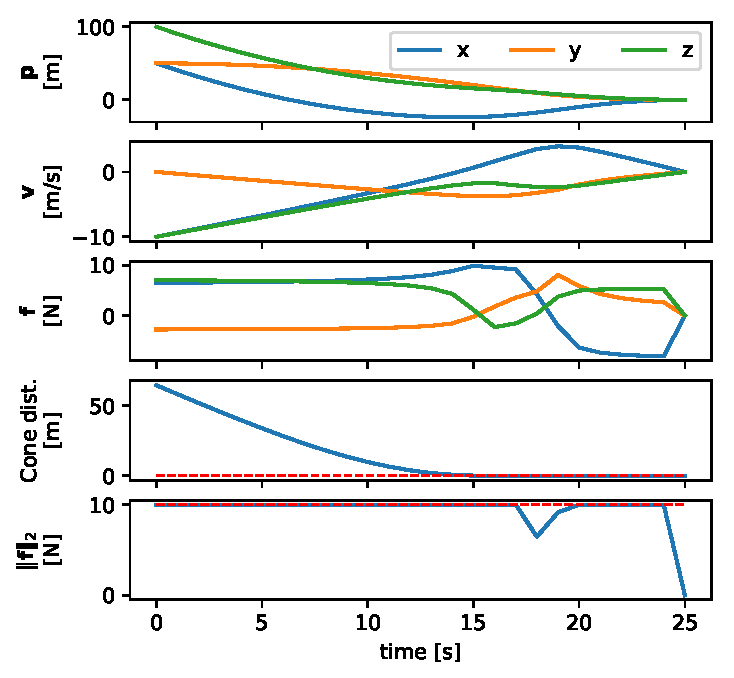
\includegraphics[width=\textwidth]{variables26.pdf}
    \caption{Evolution of position, velocity, thrust with constraint margins. $K=\SI{26}{\second}$}
    \label{fig:var26}
  \end{subfigure}
  \caption{Trajectories and variable evolution.}
  \label{fig:trandandvariables26}
\end{figure}

Comparing Figure \ref{fig:var26} with Figure \ref{fig:variables} we observe that the thrust is always active and most of the time saturated.
It is likely due to the \textit{Max Thrust} constraint that the problem becomes infeasible at $K=\SI{25}{\second}$ because the spacecraft can not accelerate and decelerate fast enough to reach the target in time.

In Figure \ref{fig:traj_multi} multiple trajectories with different feasible landing times are compared.
We notice that the trajectory for small K lead more directly to the target, while for large K the coasting phase with zero thrust is longer.
This hints at a weakness in the problem formulation: The actual landing is not modelled, where the spacecraft is supported by the ground.
Therefore, it is more fuel-efficient to enter a slow parabolic trajectory instead of heading straight to the target and hovering there until timestep K.

\subsection{Fuel Consumption}
Finally, we look at the actual fuel consumption for different landing times which is shown in figure \ref{fig:fuelconsump}.
We observe that for the minimum landing time the fuel consumption is maximal, which makes sense because hard acceleration/deceleration is costly.
However, after a certain point fuel consumption increases again for increasing $K$ because staying longer in the air requires more fuel as well.
We identify minimal fuel consumption for landing time $K=\SI{41}{\second}$.

\begin{figure}[H]
 \centering 
 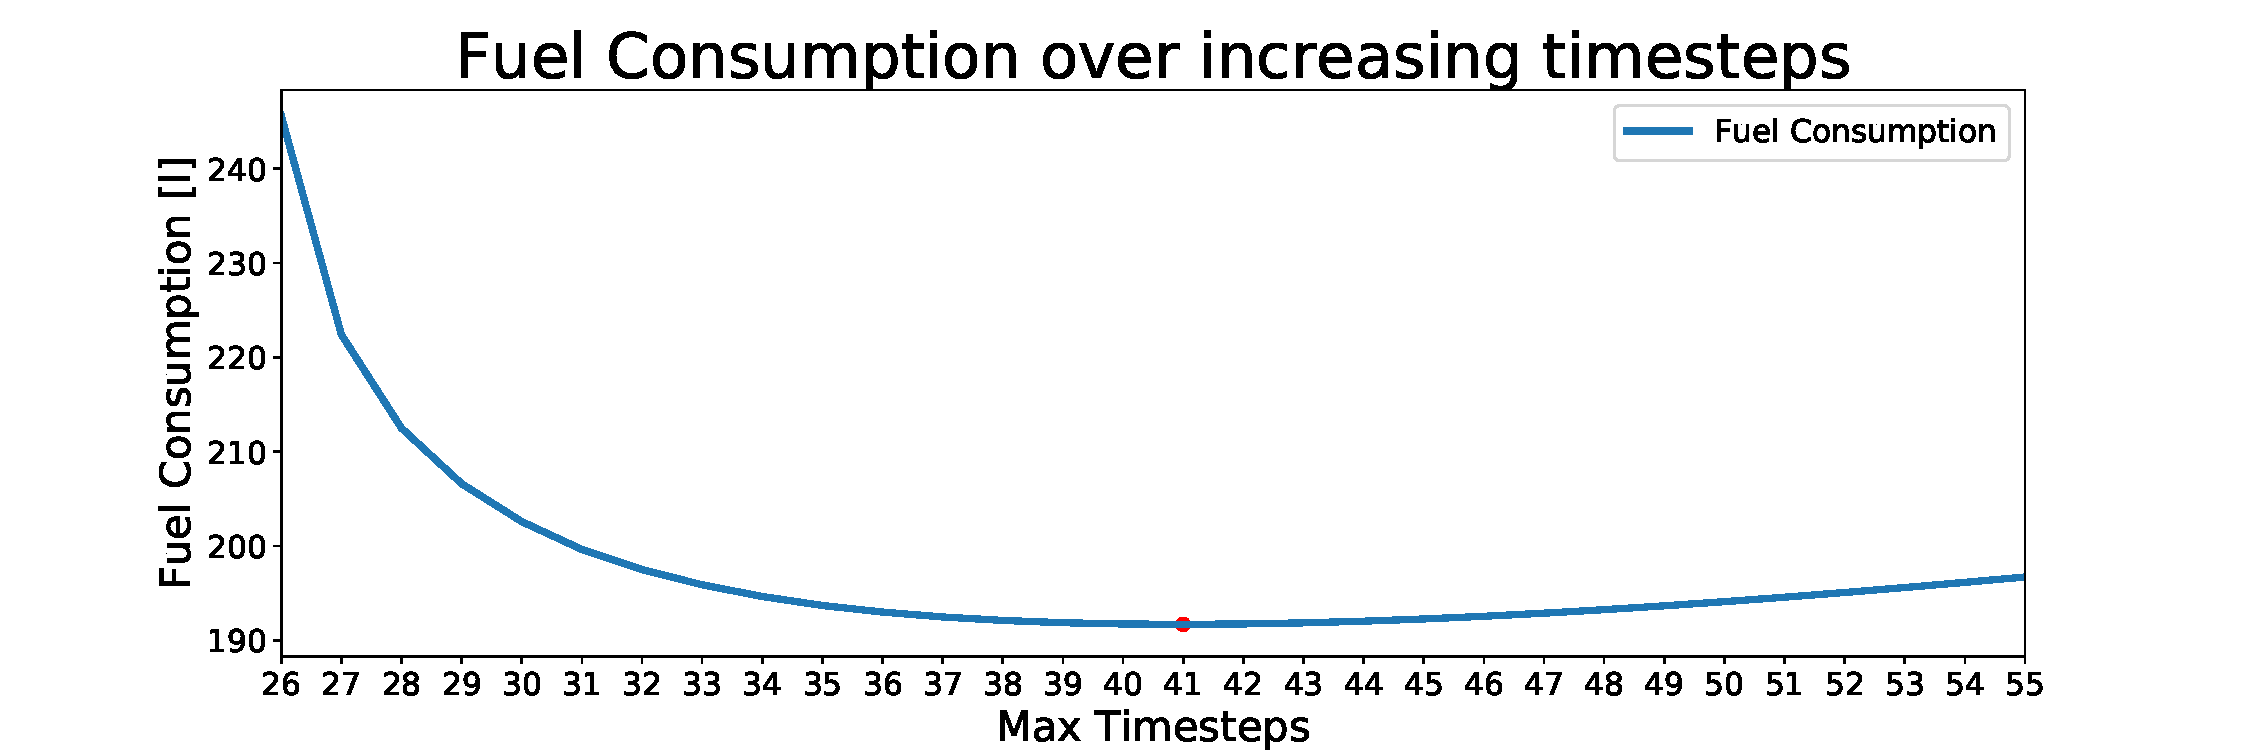
\includegraphics[width=12cm]{fuelcomsumption.pdf}
   \caption{Fuel consumption for different landing times.}
  \label{fig:fuelconsump}
\end{figure}

\section{Conclusion}
In this project we formulated and solved a minimum-fuel trajectory optimization problem for a simplified spacecraft model.
We analyzed the evolution of fuel consumption for different landing times and highlighted that the fastest landing is not the most fuel efficient.
Possible improvements could be to model the decreasing mass due fuel consumption or to model the ground supporting the spacecraft.
However, those changes could lead to a non-convex problem which CVX can not solve.
%Another more practical approach would be to develop a Model Predictive Controller (MPC) with the main goal of robusness to model uncertainty and controller stability.


\begin{thebibliography}{1}

\bibitem{Boyd:CVXcourse}
Stephen Boyd, Lieven Vandenberghe.
\textit{Convex Optimization}.
Cambridge University Press, ISBN 0521833787, 2004.

\bibitem{Boyd:CVXcourse_extra_exercises}
Stephen Boyd, Lieven Vandenberghe.
\textit{Additional Exercises for Convex Optimization}.
\url{http://web.stanford.edu/~boyd/cvxbook/bv_cvxbook_extra_exercises.pdf}

\bibitem{bib:Domahidi2013ecos}
Alexander Domahidi, Eric Chu, Stephen Boyd.
\textit{ECOS: An SOCP solver for embedded systems}.
European Control Conference (ECC), p3071-3076, 2013.

\bibitem{bib:MSL}
NASA MSL
\textit{Entry, Descent, and Landing}
Retrieved 2019 from \url{https://mars.nasa.gov/msl/mission/timeline/edl/}

\end{thebibliography}

\newpage
\appendix
\section{Matlab code}
\label{matlab_code}
\lstinputlisting[language=Matlab]{code.m}

\section{Python implementation}

While initial tests were done in Matlab, we switched to Python with CVXPY for more flexibility.
The project source code for generating the plots is published on GitHub:
\url{https://github.com/nuft/cvx-optimal-spacecraft-landing}

\end{document}
